%!TEX root = main.tex
\section{Data and User Models\label{sec:datamodel}}
\par In this section, we first describe how analysts explore the lattice through drill-downs and introduce a common fallacy that arises when analyst have limited time and attention to examine all possible factors that contribute to the observed visualization. Then, we discuss how to resolve the problem of finding informative visualizations for a given visualization.
% How users explore visualizations
% 	- Drill down
% 	- Expectation formation
% 		- focussing on bar chart 
% to explore the space of possible data subset
\par Research in visualization storytelling shows that people prefer visualization sequences structured hierarchically with increasing levels of aggregation~\cite{Kim2017,Hullman2017,Hullman2013}. In order to find the desired data subset, analysts often drill-down to explore data at different levels of granularity by adding one filter at a times. For each data subset that he encounters, he may want to visualize the distribution of measure values for each data subset through a bar chart. When analysts perform drill-downs, they naturally formulate their expectation based on the last visualization that they observe, known as the `parent', which is the visualization that can be obtained by removing one filter constraint from the current visualization in context (known as the `child' visualization). For example in Figure~\ref{fig:elections_example}, the visualizations Female and Black are the parents of the Black Female visualization. By extending this concept of parent-child relationships, we can organize the space of visualization from different data subsets to form a lattice as shown in Figure~\ref{fig:elections_example}.
\begin{figure}[h!]
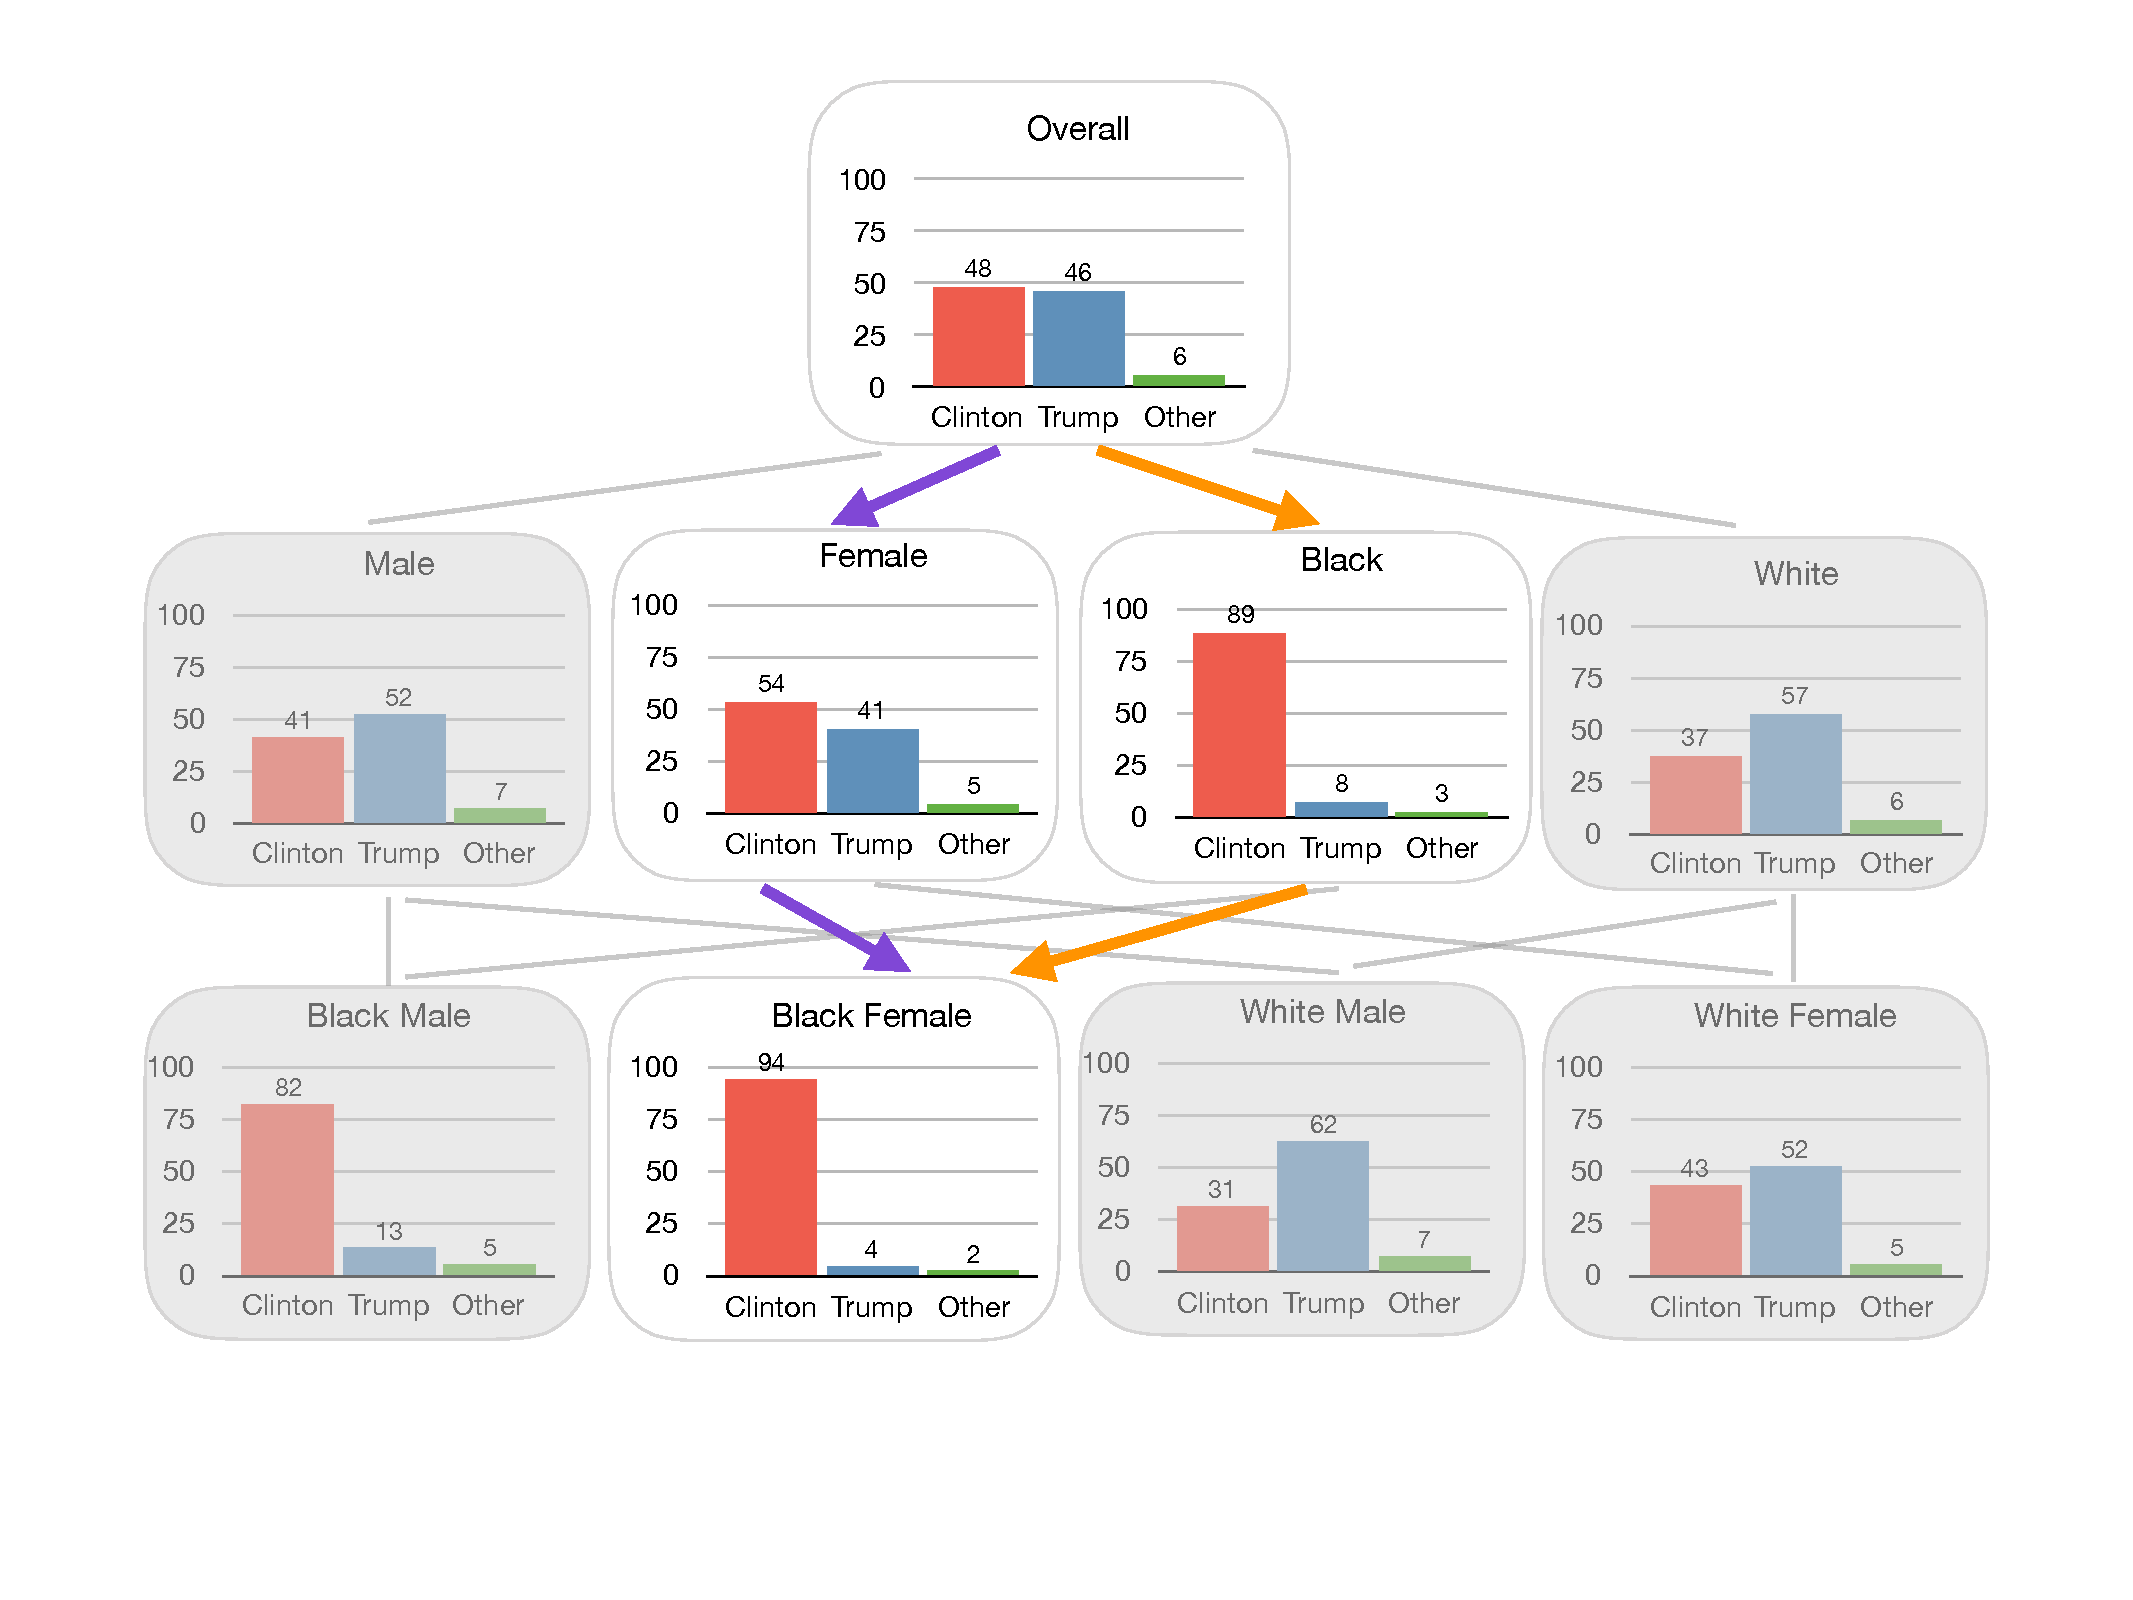
\includegraphics[width=\linewidth]{figures/elections_example_lattice.pdf}
\caption{Example data subset lattice illustrating the misleading factor fallacy along the orange path as opposed to the informative purple path.}
\label{fig:elections_example}
\end{figure}
% Fallacies of Forming Expectations:
% 	- two extremes: 
% 		- random parent v.s. exhaustive parent browsing
% 		- limitation of analyst 
\par As the analyst is drilling down by adding one filter at a time, the analyst is prone to be misguided by parent visualizations that highly deviate from its child, overlooking other potential factors that may explain the seemingly-anomalous behavior. We refer to this phenomena as \emph{drill-down fallacy}, as this type of fallacy arises from the inductive nature of the drill-down operation. We demonstrate this fallacy with an example from the 2016 US Elections exit polls dataset. As shown in Figure~\ref{fig:elections_example}, an analyst can either arrive at the Black Females visualization by going through the purple path or the orange path. At random, if the analyst went down the purple path, he may be surprised at how much the Black Female voting behavior differs drastically from the vote distribution for females. This behavior can be explained if the analyst went down the orange path, where he sees the proper reference (vote distribution for Black) that explains the behavior of the Black Female distribution. While such fallacies can be prevented if the analyst browses through all possible parents of any visualization that he observes in the dataset, the prohibitively large number of visualizations and limited memory and attention of analysts make this task impractical.
% Problem definition 
% 	- picking right parent
\par Since it is impossible to examine all possible parents and potentially misleading if we simply picked a few parents to examine, our goal is to develop a mechanism that would  \emph{provide safe guarantee by picking the proper informative parent} as a reference when analysts navigate through the space of data subsets.  To model the informativeness of an observed parent in the context of an unseen visualization, we characterize the capability of the parent in predicting the unseen visualization. An observed parent is \emph{informative} if its data distribution closely follows the data distribution of the unseen child visualization, since the visualization helps the analyst form an accurate mental picture of what to expect from the unseen visualization. Specifically, we formulate the informativeness of an observed parent $V_i^j$ of an unseen visualization $V_i$ as the similarity between their data distributions measured using a distance function $D(V_i, V_i^j)$. The most informative parents $V_i^*$ of an unseen visualization $V_i$ are the ones whose data distributions are most similar to the unseen.
\begin{equation}
    V_i^*=\underset{V_i^j}{argmin}\ D(V_i, V_i^j)
\end{equation}
We regard a visualization as informative if its distance falls within a user-defined threshold $\theta\%$ close to its most informative parent:
\begin{equation}
    V_i^{*, \theta} = \{V_i^j : \frac{D(V_i, V_i^*)}{D(V_i, V_i^j)} \geq \theta\}
\end{equation}
For example in Figure~\ref{fig:elections_example}, while both visualization Black and Female visualizations are considered parents of the Black Female visualization, only the Black visualization are considered the informative parent of the black female population, for any values of $\theta \geq 11\%$ via the Euclidean distance metric. Note that, our proposed system can work with different distance metrics such as cosine similarity and earth mover's distance. Without loss of generality, we chose to use Euclidean distance metric for the remainder of our paper.
